% Drawing 154/06-19 -- folder 154, batch 06, archive page 103 (PDF page 104).
% Transcription: petits dessins en couleur dans les lignes « le balayage de l'arc de spécialisation … donne … » et « l'antibalayage de … donne … » : un croisement de deux droites orange au-dessus de la droite vert clair ou sur elle, l'arc de spécialisation noirci et fléché ; après « donne », la droite verte contourne le croisement par-dessus (bosse en tirets), l'arc noirci passé de l'autre côté
% Kind: sweeping an arc of specialisation: before and after. Method 2 (schematic redraw from the facsimile). Status: partial.
% Notes: Three lines of the text carry a sketch before and after the word « donne » (the word itself belongs to the text). First line: a crossing above the light green line, the arc of the line between its legs black, a small arrow up; then the line (dark green at first) rising in dashes over the crossing and coming down, a short dark stroke on top of the crossing, an arrow down. Second line: the crossing on the line, a black stroke between the legs below it, a double arrow; then the dashed bump over the crossing, a second row of dashes below, the black stroke above the crossing, an arrow down. Third line (antibalayage): a crossing on the line, over-inked in green on the page and drawn plain here, an arrow to the left, and a crossing above the line with the black arc between its legs. Crossing points computed, black arcs drawn between the legs. Redrawn 2026-11-12 (issue 128): to check again.
% Coordinates: 1 unit = 1 mm = 1/100 of the crop width (bbox in page fractions: [0.665, 0.23, 0.91, 0.32]).
% Redrawn by Claude (claude-fable-5-2), issue #128, 2026-11-12; not checked by a human; not compiled (no TeX in the session).
% Rights: reproduces part of the work -- behind RENDER_TRANSCRIPTS, never published by itself.
\documentclass[tikz,border=3pt]{standalone}
\usepackage{amsmath,amssymb}
\usetikzlibrary{patterns,arrows.meta}
\tikzset{Or/.style={orange!90!black}, Lg/.style={green!60!black!70}, Dg/.style={green!45!black}, Bl/.style={blue!70!black}, pencil/.style={black!45}, struck/.style={black!35}, mpt/.style={circle,draw,inner sep=1.3pt}, pt/.style={circle,fill,inner sep=0.9pt}, opt/.style={circle,draw,fill=white,inner sep=1.1pt}}
\begin{document}
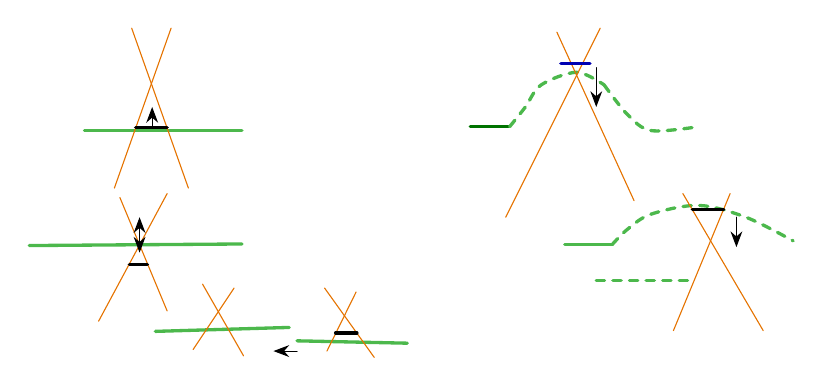
\begin{tikzpicture}[x=1mm,y=1mm,line cap=round,line join=round,font=\scriptsize]
\draw[Lg,very thick] (10,-19) -- (30,-19);
\draw[Or] (16,-6) -- (23.2,-26.3);
\draw[Or] (21,-6) -- (13.8,-26.3);
\draw[very thick] (16.5,-18.6) -- (20.5,-18.6);
\draw[-{Stealth[length=2mm]}] (18.6,-18.4) -- (18.6,-16);
\draw[Dg,very thick] (59,-18.5) -- (64,-18.5);
\draw[Lg,dashed,very thick] plot[smooth, tension=0.55] coordinates {(64,-18.5) (66,-16) (68,-13.2) (72.5,-11.6) (76,-13.2)};
\draw[Lg,dashed,very thick] plot[smooth, tension=0.55] coordinates {(76,-13.2) (79,-17) (82,-19) (88,-18.5)};
\draw[Or] (70,-6.5) -- (79.8,-27.9);
\draw[Or] (75.5,-6) -- (63.5,-30);
\draw[Bl,very thick] (70.5,-10.5) -- (74.2,-10.5);
\draw[-{Stealth[length=2mm]}] (75,-11) -- (75,-16);
\draw[Lg,very thick] (3,-33.6) -- (30,-33.4);
\draw[Or] (14.5,-27.5) -- (20.5,-41.9);
\draw[Or] (20.5,-27) -- (11.8,-43.2);
\draw[very thick] (15.7,-36) -- (18,-36);
\draw[{Stealth[length=2mm]}-{Stealth[length=2mm]}] (17,-34.5) -- (17,-30);
\draw[Lg,very thick] (71,-33.5) -- (77,-33.5);
\draw[Lg,dashed,very thick] plot[smooth, tension=0.55] coordinates {(77,-33.5) (79,-31.5) (82,-29.6) (88,-28.5) (94,-30) (100,-33)};
\draw[Lg,dashed,very thick] (75,-38) -- (87,-38);
\draw[Or] (86,-27) -- (96.2,-44.4);
\draw[Or] (92,-27) -- (84.8,-44.4);
\draw[very thick] (87.2,-29) -- (91.2,-29);
\draw[-{Stealth[length=2mm]}] (92.8,-30) -- (92.8,-33.8);
\draw[Lg,very thick] (19,-44.5) -- (36,-44);
\draw[Or] (25,-38.5) -- (30.2,-47.6);
\draw[Or] (29,-39) -- (23.8,-46.8);
\draw[-{Stealth[length=2mm]}] (37,-47) -- (34,-47);
\draw[Lg,very thick] (37,-45.7) -- (51,-46);
\draw[Or] (40.5,-39) -- (46.8,-47.8);
\draw[Or] (44.5,-39.5) -- (40.8,-47);
\draw[very thick] (41.9,-44.7) -- (44.6,-44.7);
\end{tikzpicture}
\end{document}
